\documentclass{article}
\usepackage[utf8]{inputenc}
\usepackage[spanish]{babel}
\usepackage{listingsutf8}
\usepackage{xcolor}
\usepackage{pdfpages}
\usepackage{geometry}
%\usepackage{hyperref}

\geometry{
    a4paper,
    margin=1.2in
}

\title{Procesos Estocásticos (66.75): Trabajo Práctico n.1}
\author{
    Cáceres, Julieta (\texttt{\#})\\\texttt{}\\
    Rozanec, Matias (\texttt{\#97404})\\\texttt{rozanecm@gmail.com}}
\date{8.mayo.2018}

\begin{document}
\maketitle
\newpage

\tableofcontents
\newpage

% *** ENUNCIADO ***
% \part{Enunciado}
% 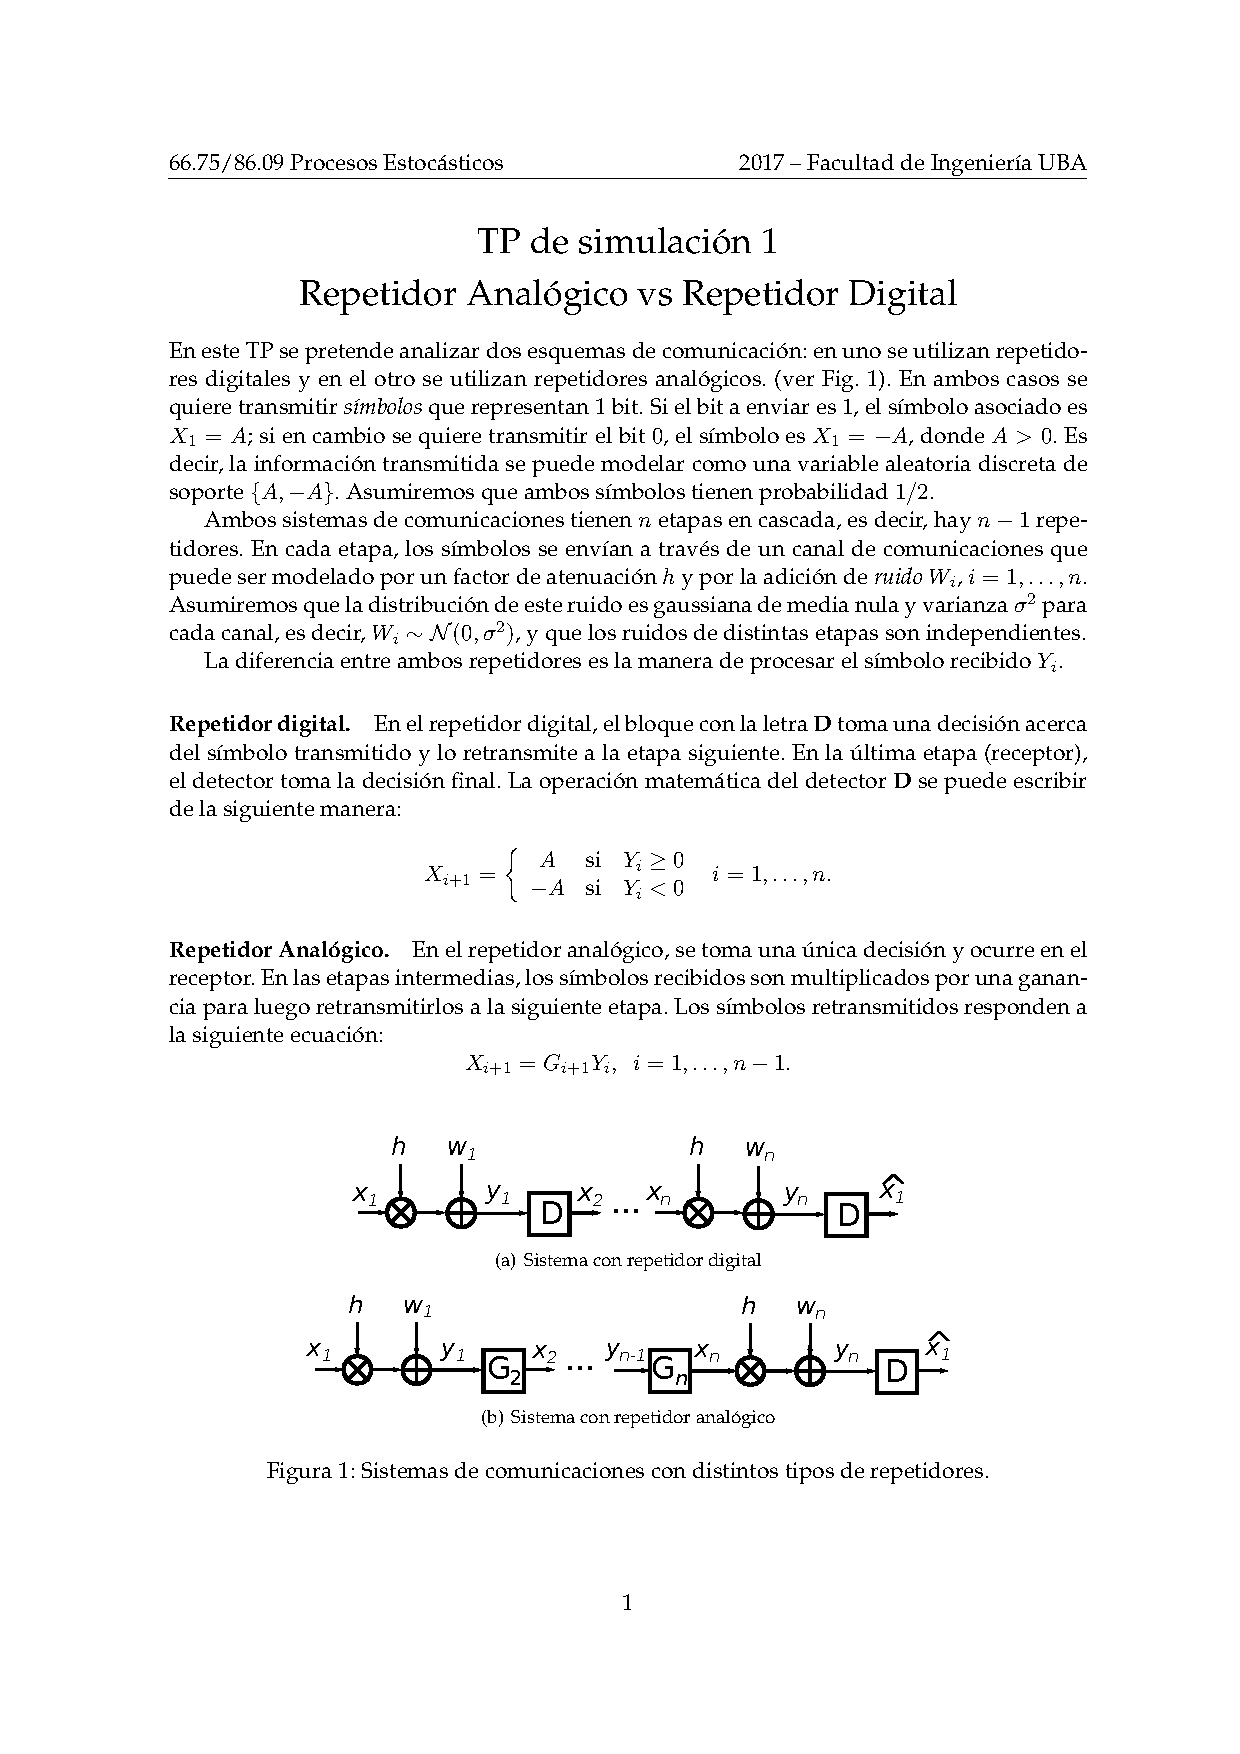
\includepdf[pages=-]{Enunciado.pdf}

% *** RESOLUCION ***
% Some settings for coding style
\lstset{
    basicstyle=\linespread{0.9}\ttfamily\footnotesize,
    frame=single,
    frameround=tttt,
    numbers=left,
    numberstyle=\tiny,
    linewidth=14cm,
    literate=
      {á}{{\'a}}1 {é}{{\'e}}1 {í}{{\'i}}1 {ó}{{\'o}}1 {ú}{{\'u}}1
      {Á}{{\'A}}1 {É}{{\'E}}1 {Í}{{\'I}}1 {Ó}{{\'O}}1 {Ú}{{\'U}}1
      {à}{{\`a}}1 {è}{{\`e}}1 {ì}{{\`i}}1 {ò}{{\`o}}1 {ù}{{\`u}}1
      {À}{{\`A}}1 {È}{{\'E}}1 {Ì}{{\`I}}1 {Ò}{{\`O}}1 {Ù}{{\`U}}1
      {ä}{{\"a}}1 {ë}{{\"e}}1 {ï}{{\"i}}1 {ö}{{\"o}}1 {ü}{{\"u}}1
      {Ä}{{\"A}}1 {Ë}{{\"E}}1 {Ï}{{\"I}}1 {Ö}{{\"O}}1 {Ü}{{\"U}}1
      {â}{{\^a}}1 {ê}{{\^e}}1 {î}{{\^i}}1 {ô}{{\^o}}1 {û}{{\^u}}1
      {Â}{{\^A}}1 {Ê}{{\^E}}1 {Î}{{\^I}}1 {Ô}{{\^O}}1 {Û}{{\^U}}1
      {œ}{{\oe}}1 {Œ}{{\OE}}1 {æ}{{\ae}}1 {Æ}{{\AE}}1 {ß}{{\ss}}1
      {ű}{{\H{u}}}1 {Ű}{{\H{U}}}1 {ő}{{\H{o}}}1 {Ő}{{\H{O}}}1
      {ç}{{\c c}}1 {Ç}{{\c C}}1 {ø}{{\o}}1 {å}{{\r a}}1 {Å}{{\r A}}1
      {€}{{\euro}}1 {£}{{\pounds}}1 {«}{{\guillemotleft}}1
      {»}{{\guillemotright}}1 {ñ}{{\~n}}1 {Ñ}{{\~N}}1 {¿}{{?`}}1
}
\part{Resolución}
\section{Ejercicio 1: Cálculo de ganancia de los repetidores analógicos}
\iffalse
Por definición, la energía promedio de cada repetidor es la varianza de la variable aleatoria asociada, es decir que
\begin{equation}
    V(X_{r+1})=V(h G_{r+1} X_r + G_{r+1} W_r)
\end{equation}
Como son variables descorrelacionadas, vale que la expresión anterior es equivalente a:
\begin{equation}\label{eq:2}
    V(h G_{r+1} X_r) + V(G_{r+1}W_r)=h^2 G_{r+1}^2 V(X_r) + G_{r+1}^2 V(W_r)
\end{equation}

La varianza de $X_r$ se calcula como
\begin{equation}\label{var_X_r}
    V(X_r)=E[X_r^2]+E[X_r]^2
\end{equation}

\begin{equation}\label{esperanza_X_r_cuadrado}
    E[X_r^2]=(A^2 p(A)+(-A)^2p(-A))=(A^2\frac{1}{2}+A^2\frac{1}{2})=A^2=A^2
\end{equation}

\begin{equation}\label{esperanza_X_r}
    E[X_r]^2=(Ap(A)+(-A)p(-A))^2=(A\frac{1}{2}-A\frac{1}{2})^2=0^2=0
\end{equation}

Con \ref{esperanza_X_r} y \ref{esperanza_X_r_cuadrado} en \ref{var_X_r}:

\begin{equation}\label{var_X_r_completa}
    V(X_r)=A^2
\end{equation}

Con \ref{var_X_r_completa} en \ref{eq:2}:

\begin{equation}
    V(X_{r+1})=h^2 G_{r+1}^2 A^2 + G_{r+1} ^2 \sigma ^2 = G_{r+1}^2(h^2 A^2 + \sigma ^2)
\end{equation}
\fi

\begin{equation}
    \varepsilon_{X_i}=Var(X_i)=E(X_i^2)+E(X_i)^2
\end{equation}

\begin{equation}\label{esperanza_X_r_cuadrado}
    E[X_r^2]=(A^2 p(A)+(-A)^2p(-A))=(A^2\frac{1}{2}+A^2\frac{1}{2})=A^2=A^2
\end{equation}

\begin{equation}\label{esperanza_X_r}
    E[X_r]^2=(Ap(A)+(-A)p(-A))^2=(A\frac{1}{2}-A\frac{1}{2})^2=0^2=0
\end{equation}

Por lo tanto, 
\begin{equation}
    \varepsilon_{X_i}=A^2 \Leftrightarrow A=\sqrt{\varepsilon_{X_i}}
\end{equation}

Como $X_n = G_i X_{i-1} h + G_i W_{i-1}$, entonces:
\begin{equation}
    \varepsilon_n=Var(X_n)=(G_i h)^2 Var(X_{i-1})+G_i^2 \sigma ^2
\end{equation}

Por enunciado vale que $\varepsilon_i = \varepsilon_{i-1}$, por lo tanto
\begin{equation}
    \varepsilon_n = (G_i h)^2 \varepsilon_i + G_i^2 \sigma ^2 \Leftrightarrow \frac{\varepsilon_n}{h^2 \varepsilon_i + \sigma ^2}=G_i^2 \Leftrightarrow G_i=\sqrt{\frac{\varepsilon_n}{h^2 \varepsilon_i + \sigma ^2}}
\end{equation}
Por lo tanto, se tiene que 
\begin{equation}
    G_i=\frac{1}{h}\sqrt{\frac{SNR}{SNR+1}}
\end{equation}

\newpage
\section{Ejercicio 2: Probabilidad de error del sistema analógico}

\newpage
\section{Ejercicio 3: Probabilidad de error del sistema digital}

\newpage
\section{Ejercicio 4: Simulación Monte Carlo de las probabilidades de error}
\end{document}
